\begin{figure}[p]
    \centering
    \begin{minipage}[b]{.48\textwidth}
        \begin{figure}[H]
            \centering
            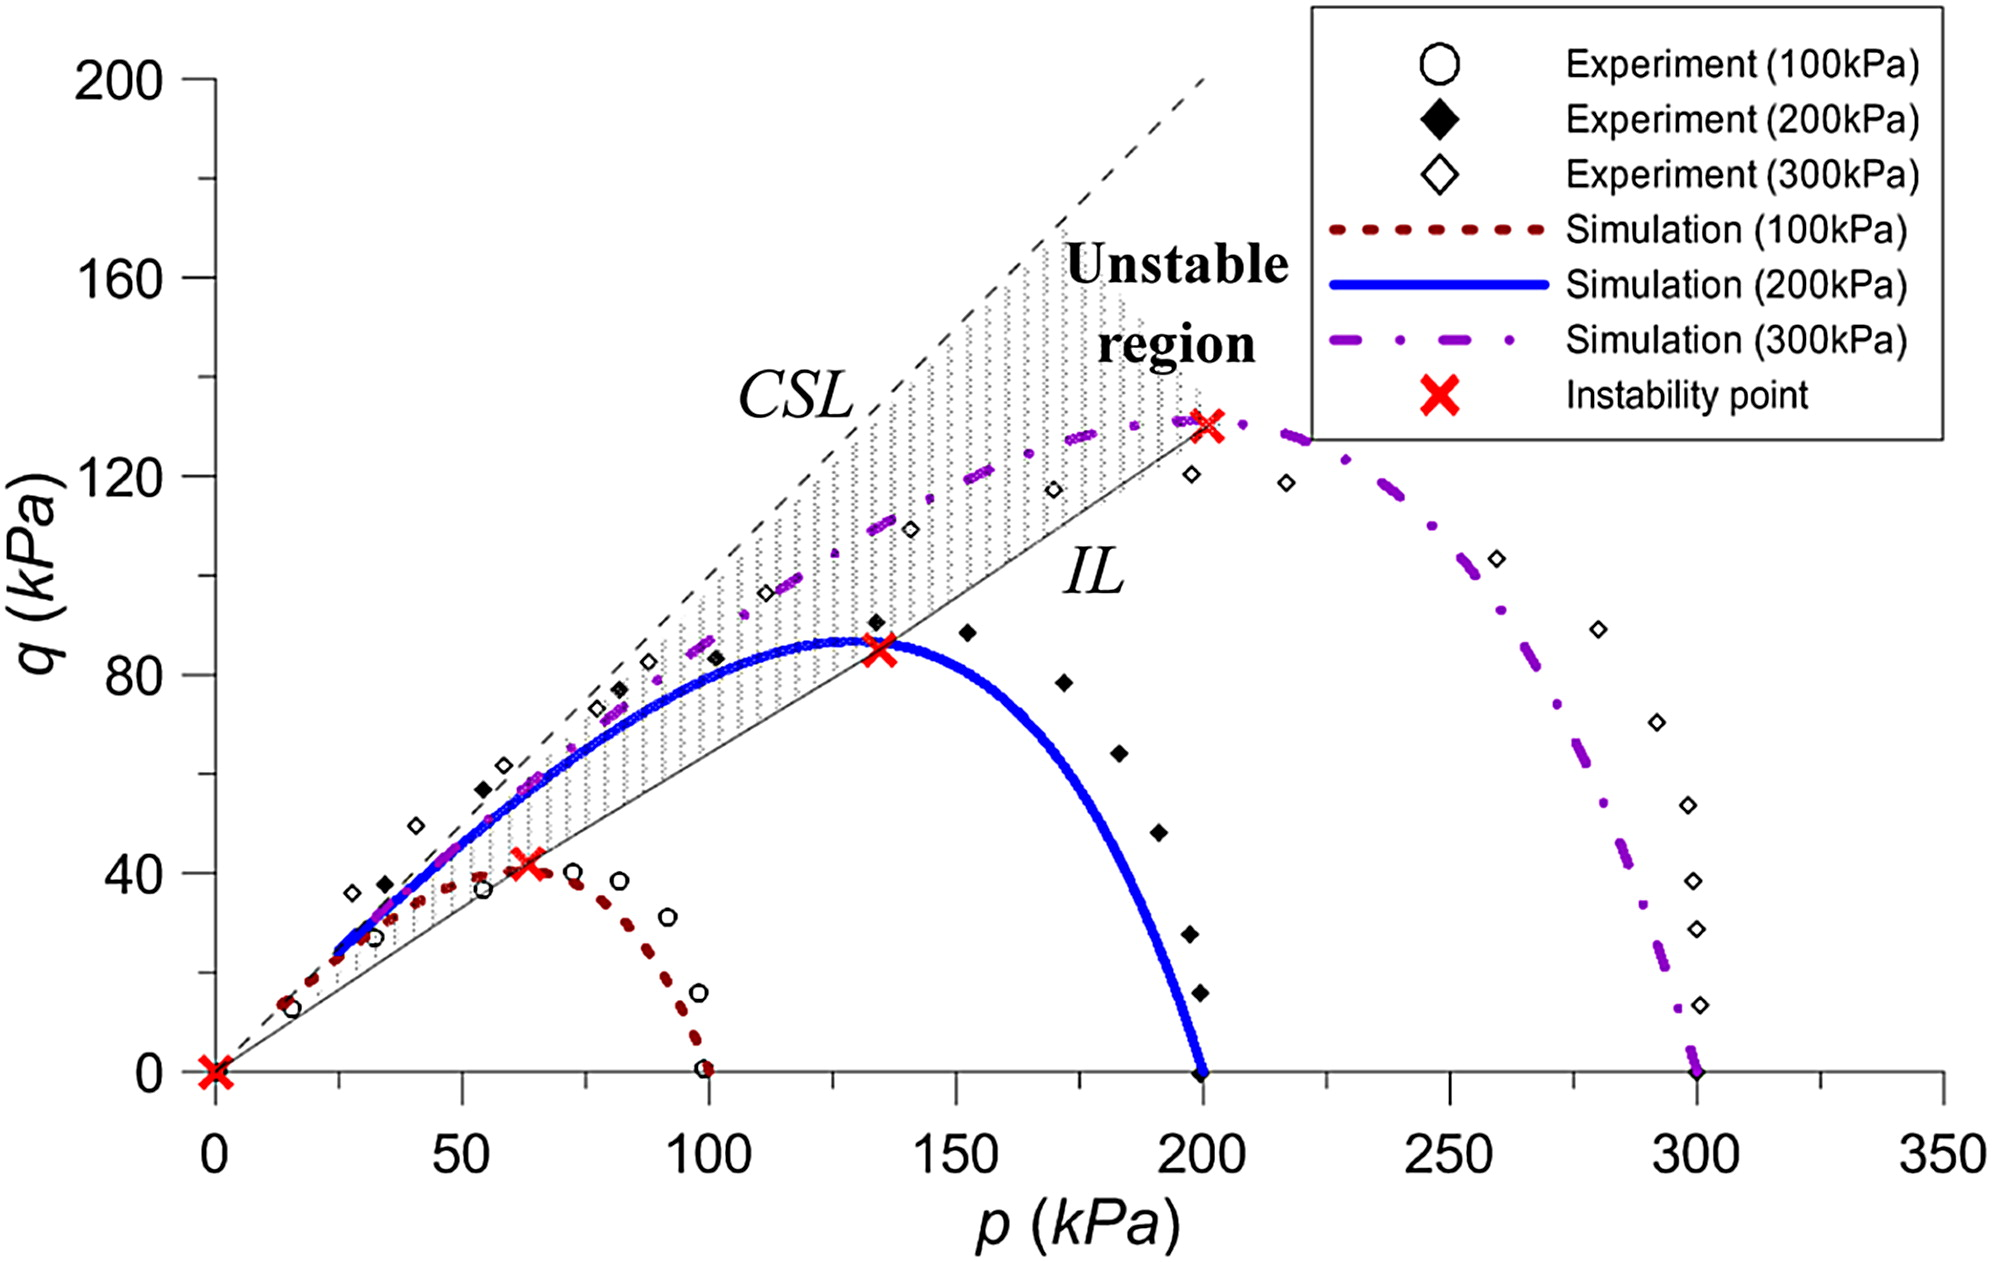
\includegraphics[width=.75\textwidth]{figures/figure4.jpg}
            \bicaption{Stress path of isotropically consolidated undrained triaxial test (experimental data from \citet{Doanh1997})}{各向同性固结不排水三轴试验的应力路径(实验数据来自\citet{Doanh1997})}
            \label{figure:4}
        \end{figure}
        \begin{figure}[H]
            \centering
            \addtocounter{figure}{1}
            \subfigure[determinant of the symmetric part of the elastoplastic modulus tensor 弹塑性模量张量的对称部分的行列式的演变]{
                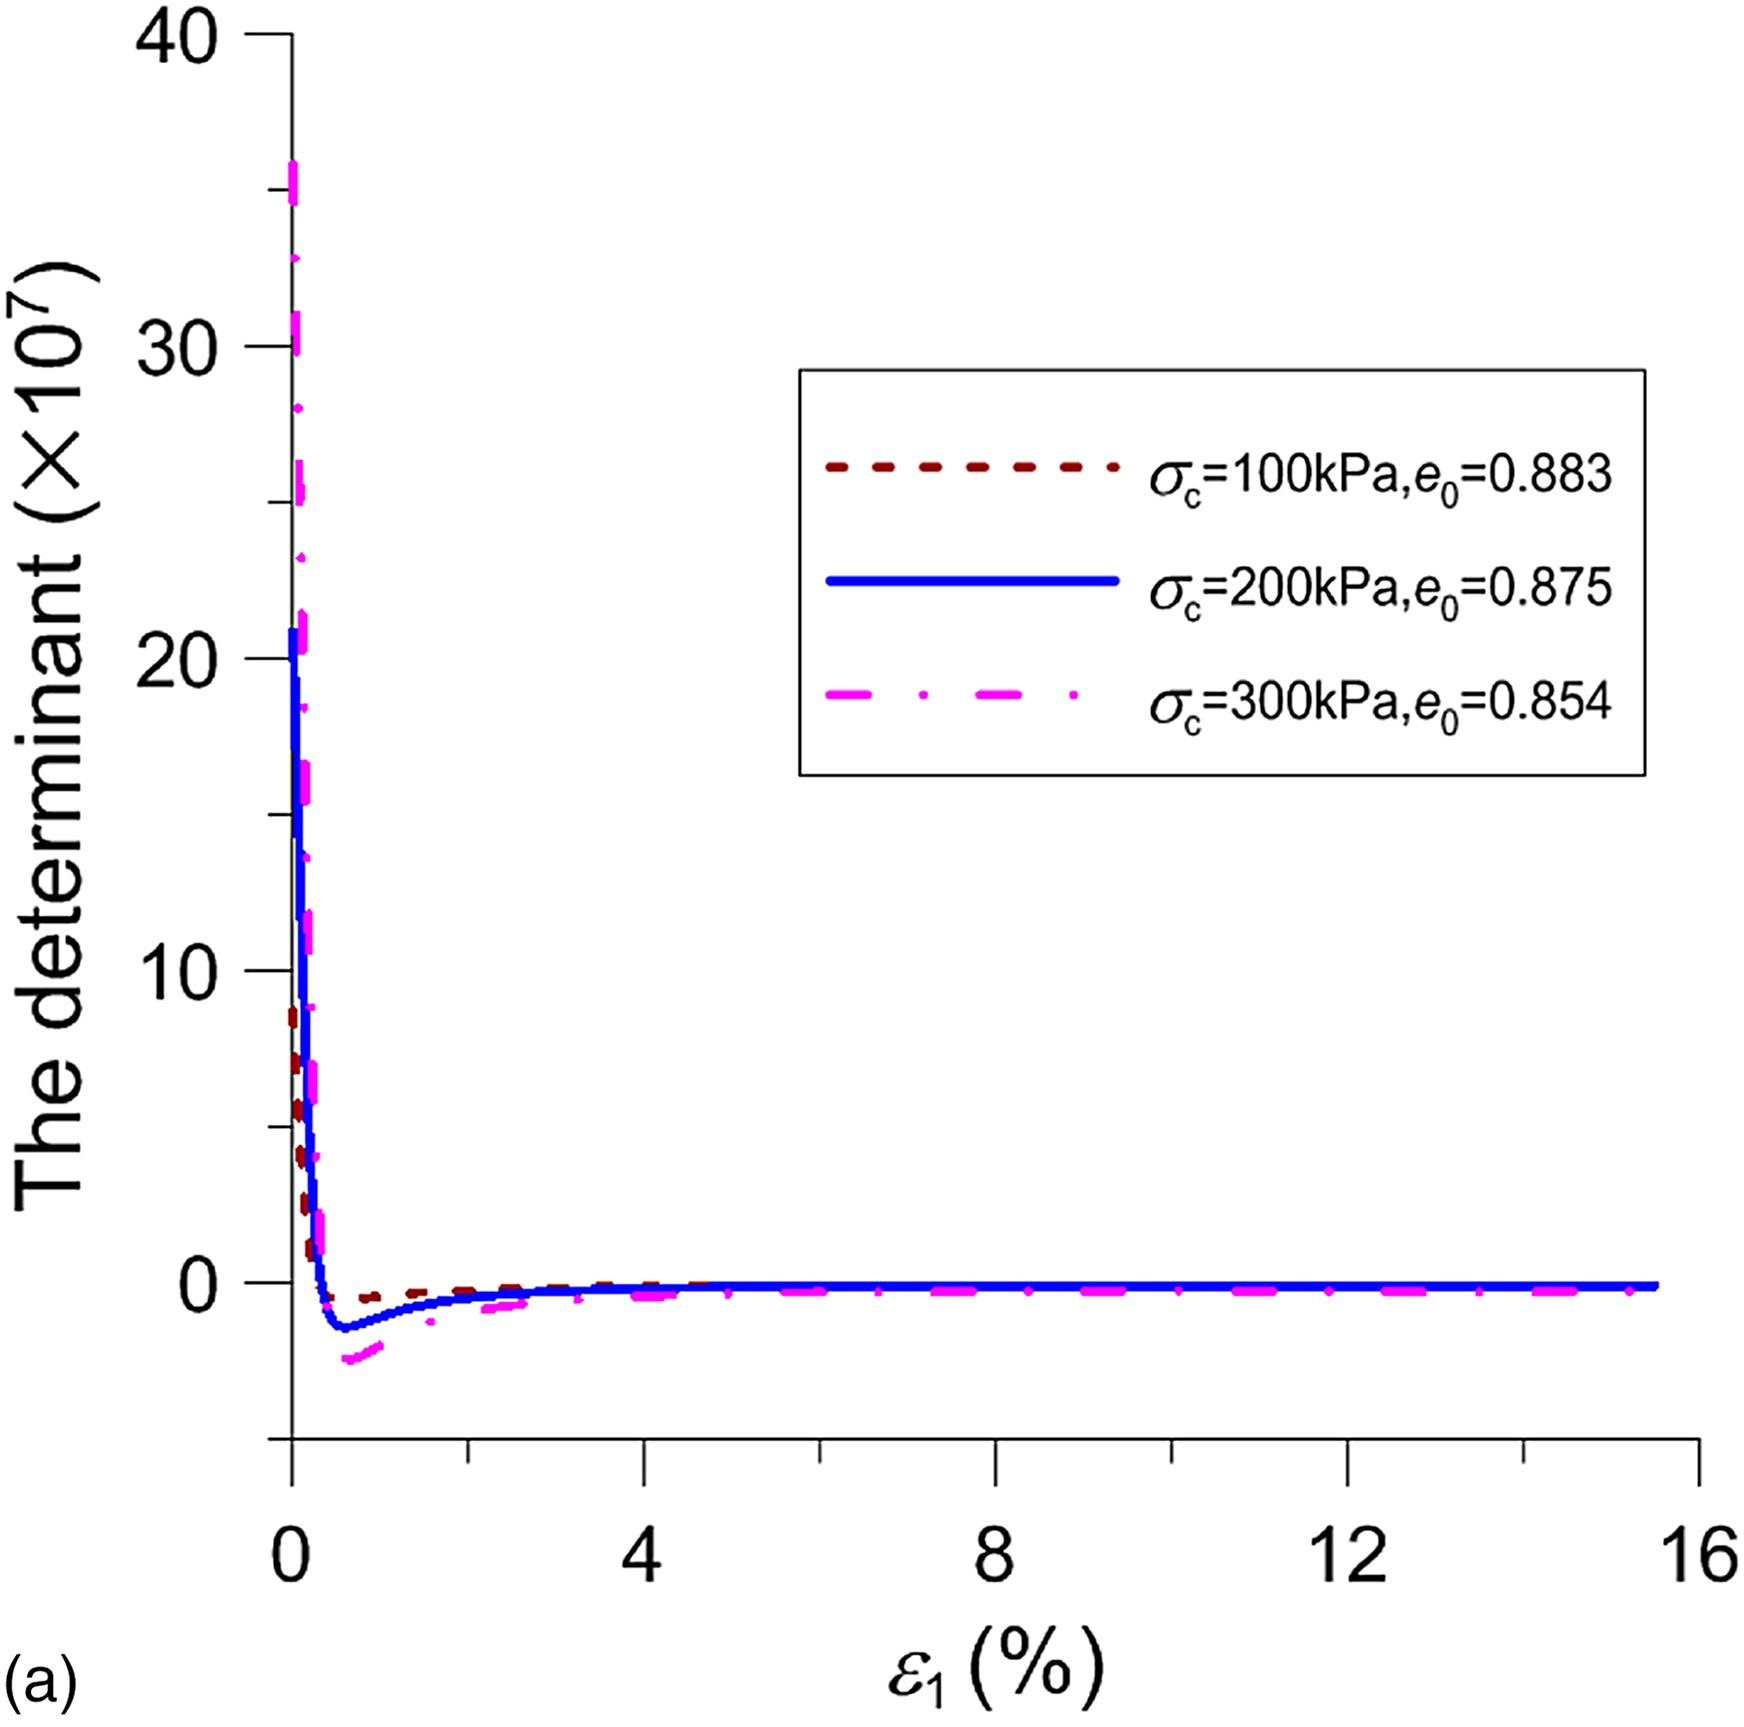
\includegraphics[width=.75\textwidth]{figures/figure6a.jpg}
                \label{figure:6a}
            }
            \subfigure[evolution of second-order work 二阶功]{
                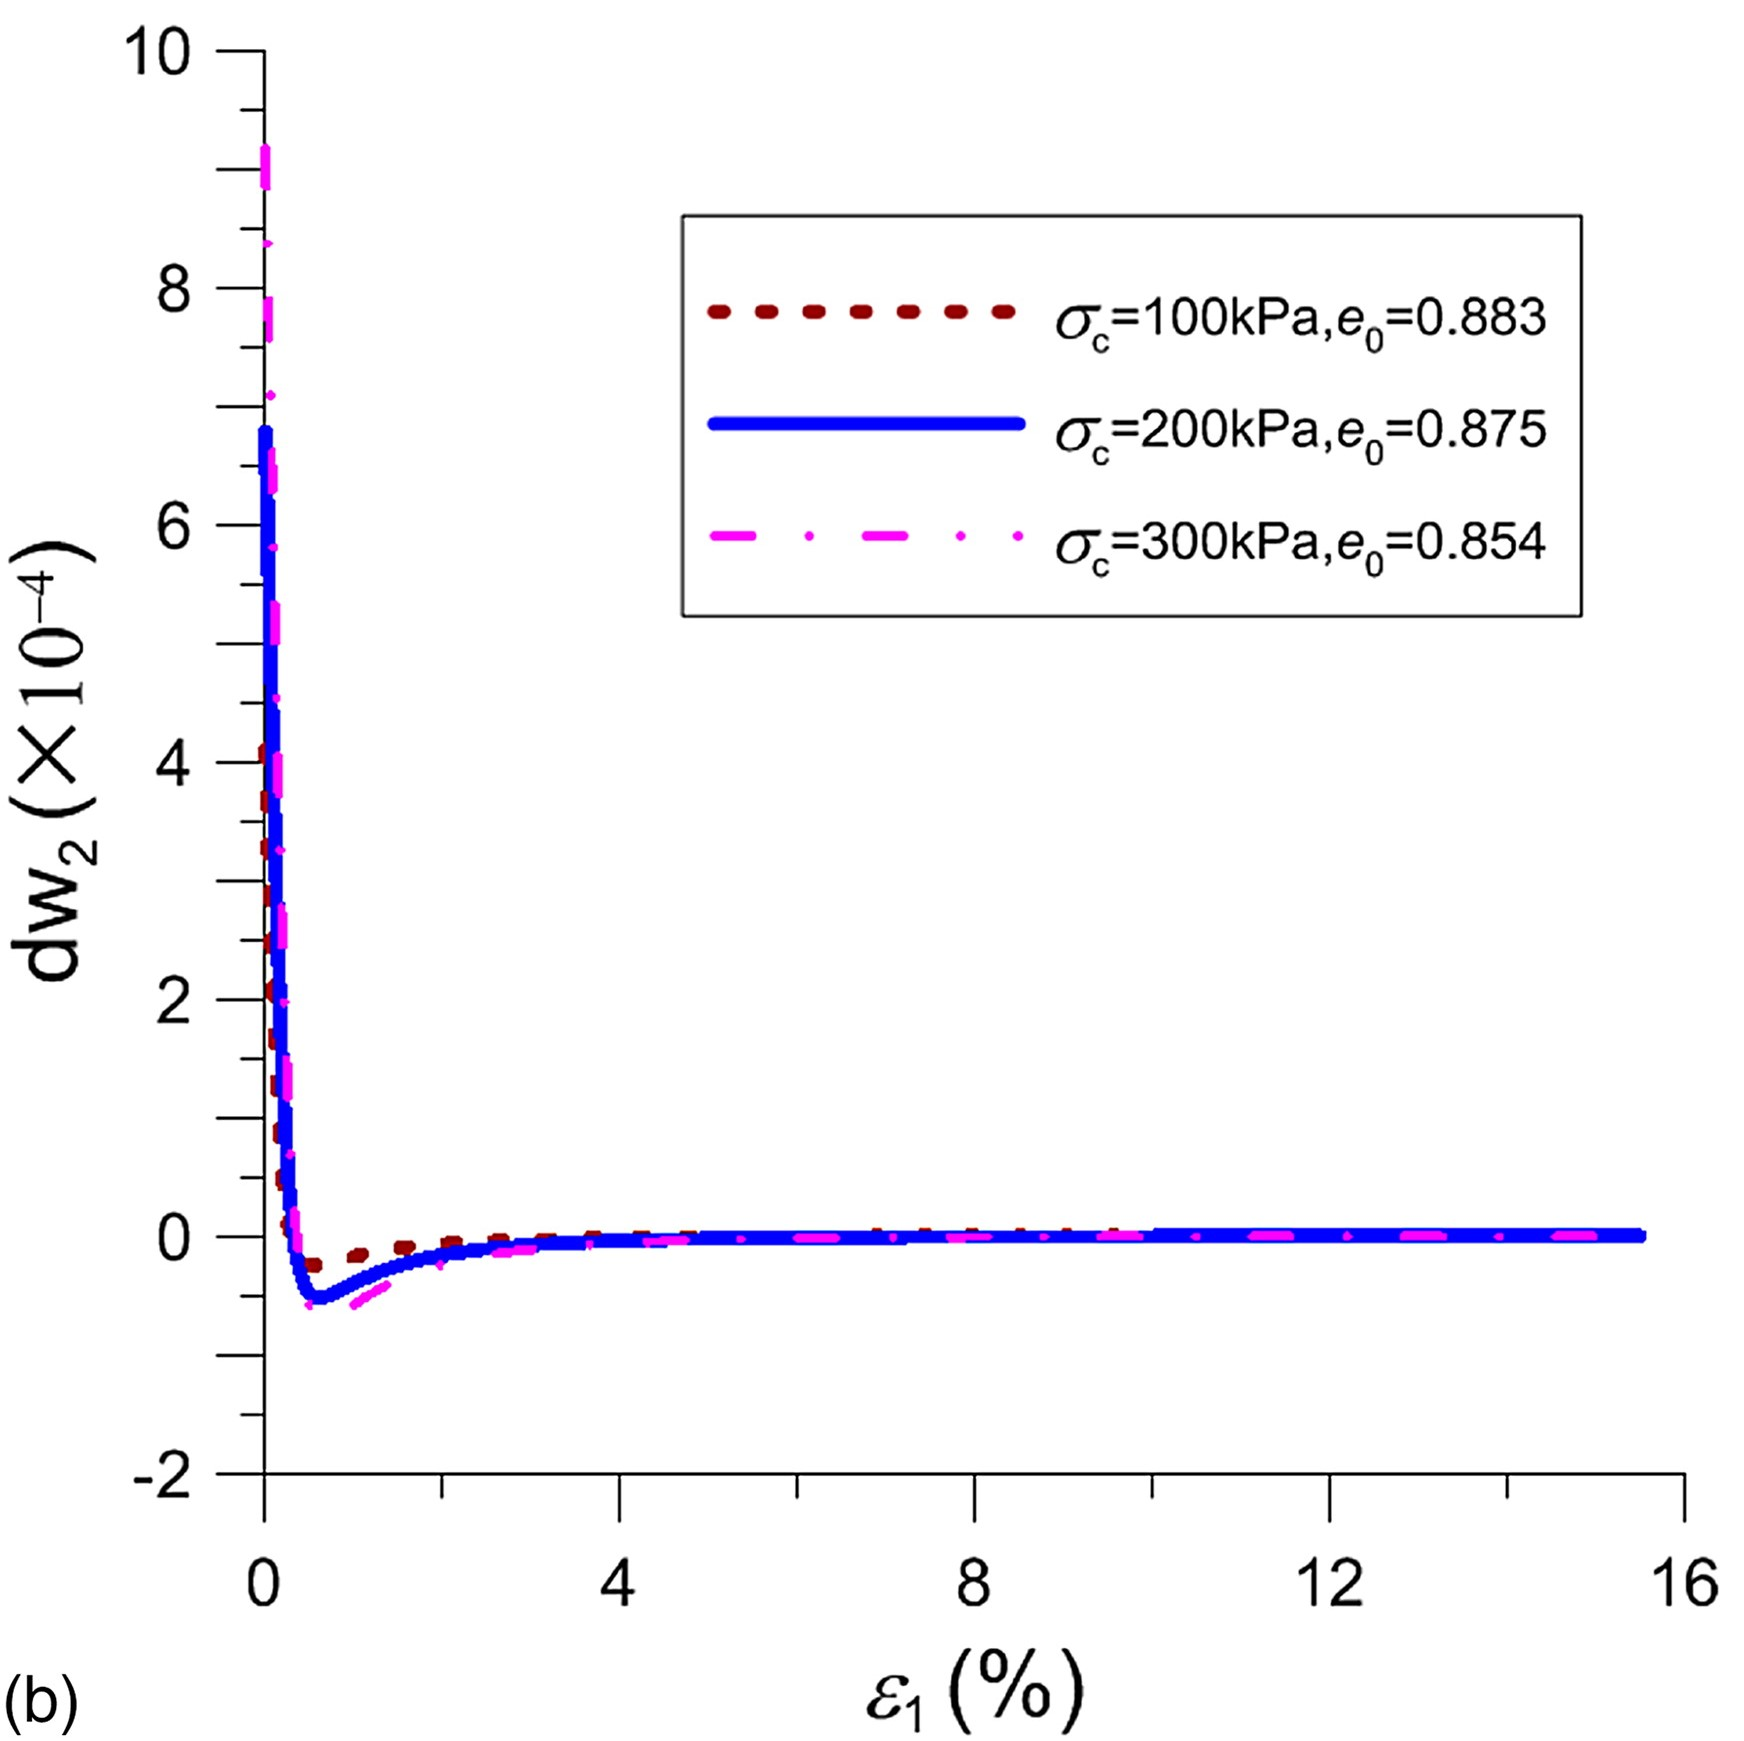
\includegraphics[width=.75\textwidth]{figures/figure6b.jpg}
                \label{figure:6b}
            }
            \bicaption{Evolution of determinant of the symmetric part of the elastoplastic modulus tensor and second-order work}{弹塑性模量张量的对称部分的行列式的和二阶功的演变}
            \label{figure:6}
        \end{figure}
    \end{minipage}
    \hspace{0.02\textwidth}
    \begin{minipage}[b]{.48\textwidth}
        \begin{figure}[H]
            \centering
            \addtocounter{figure}{-2}
            \subfigure[deviatoric stress, major principal strain 偏应力,主应变]{
                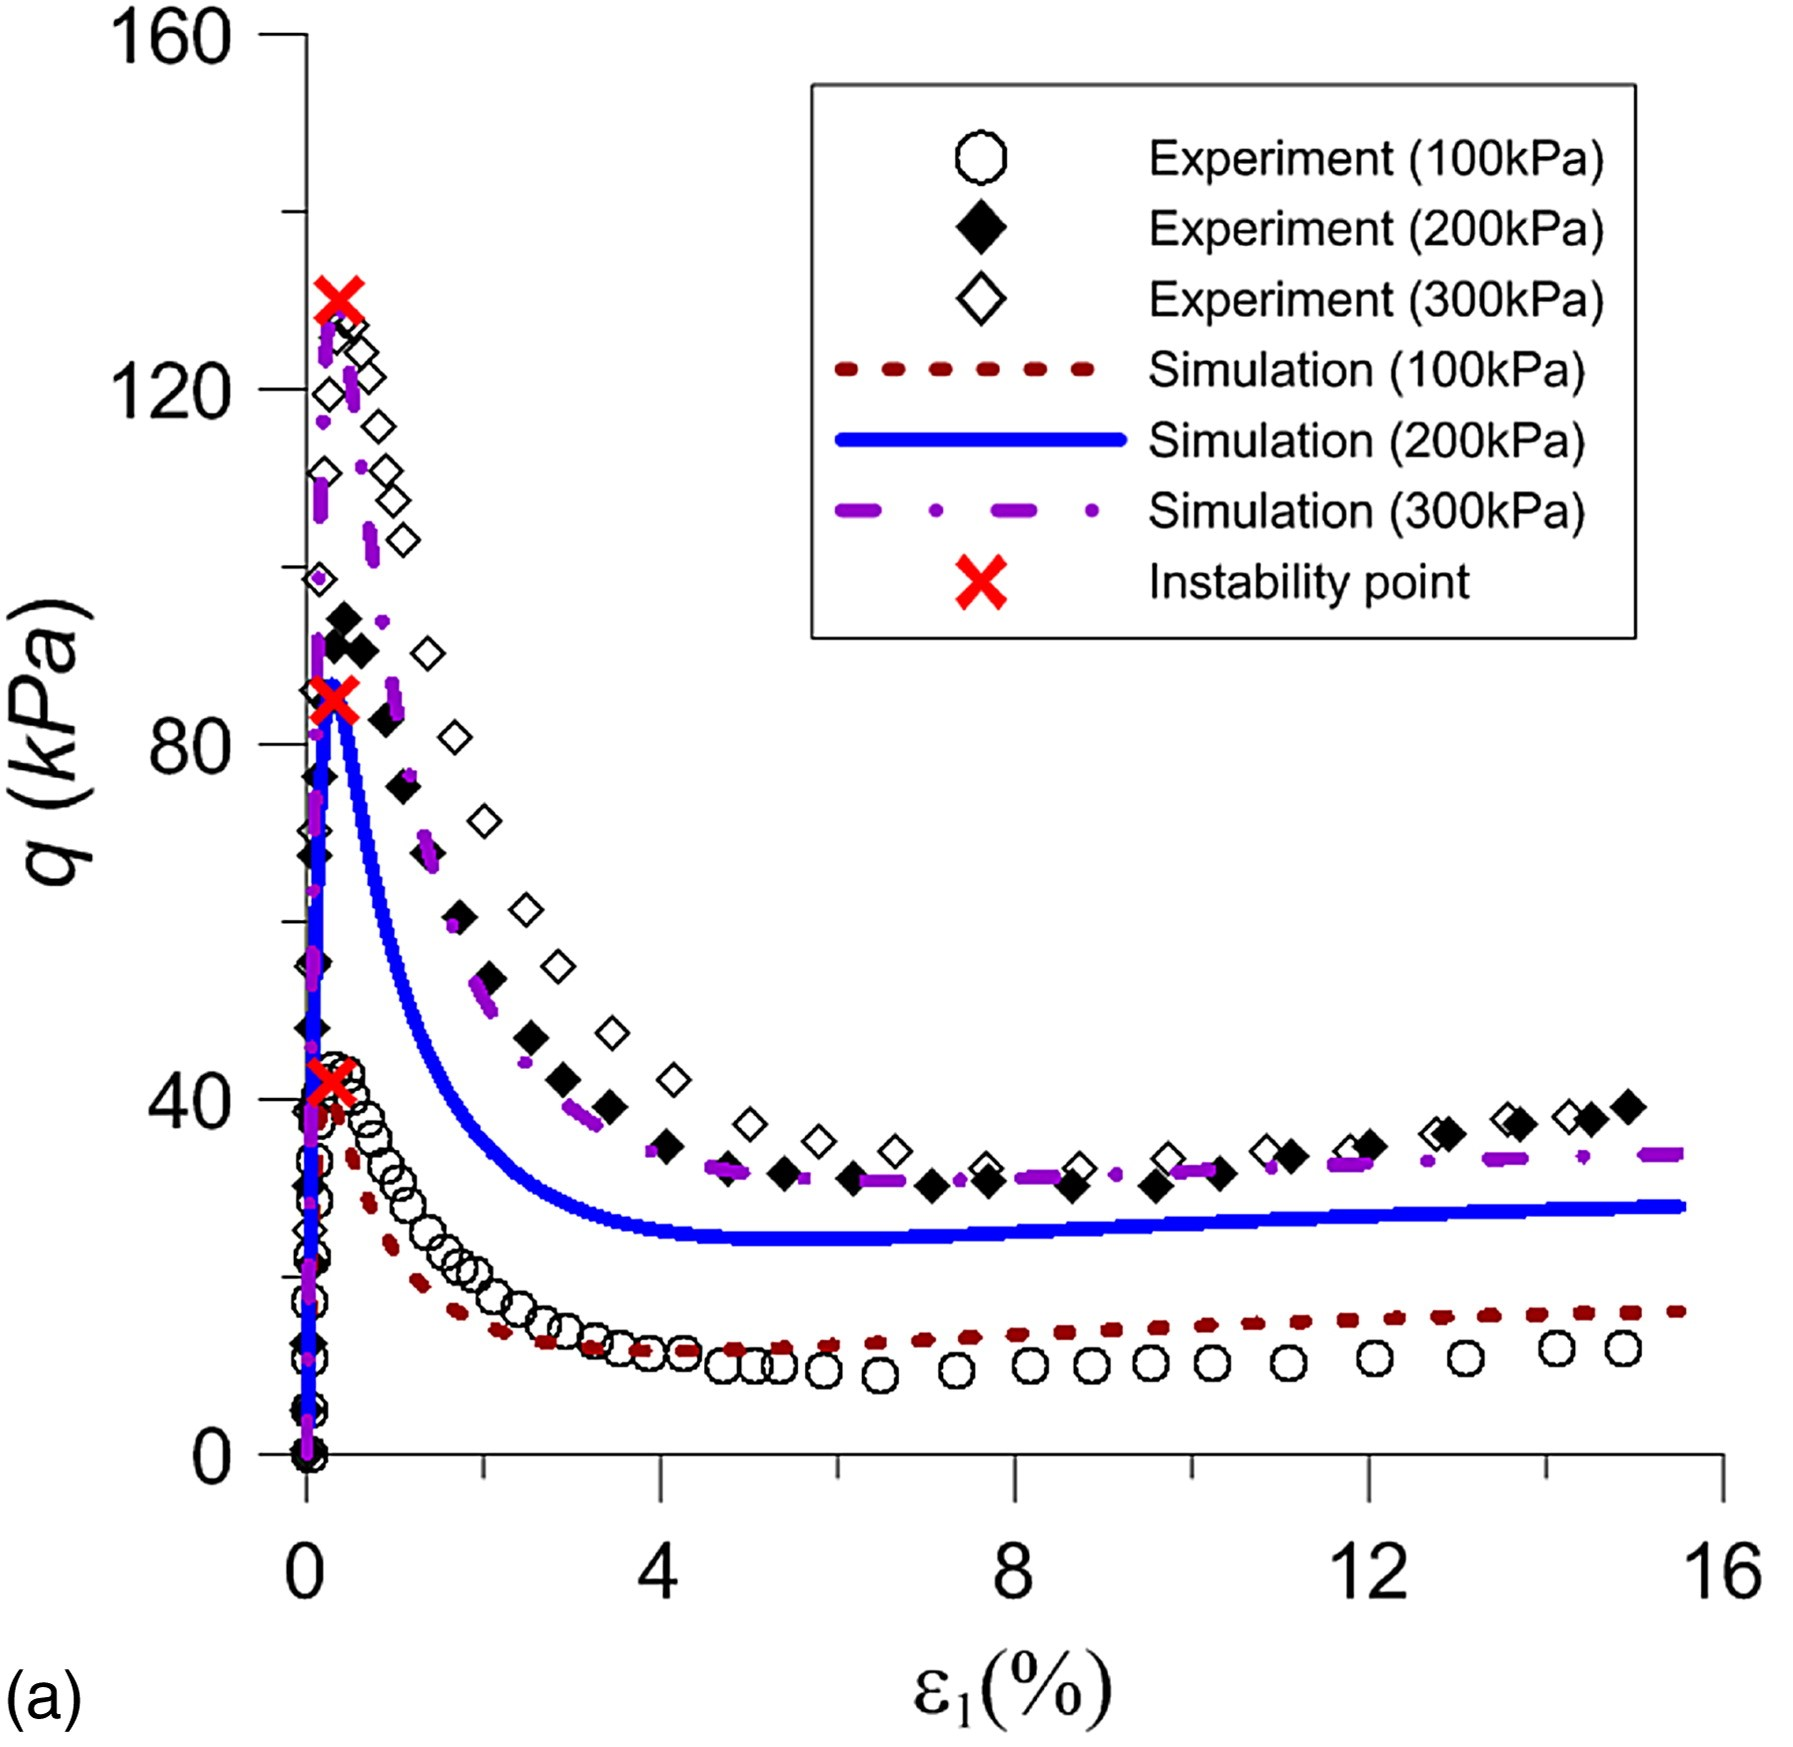
\includegraphics[width=.75\textwidth]{figures/figure5a.jpg}
                \label{figure:5a}
            }
            \subfigure[normalized pore pressure, major principal strain 归一化孔隙水压力,主应变]{
                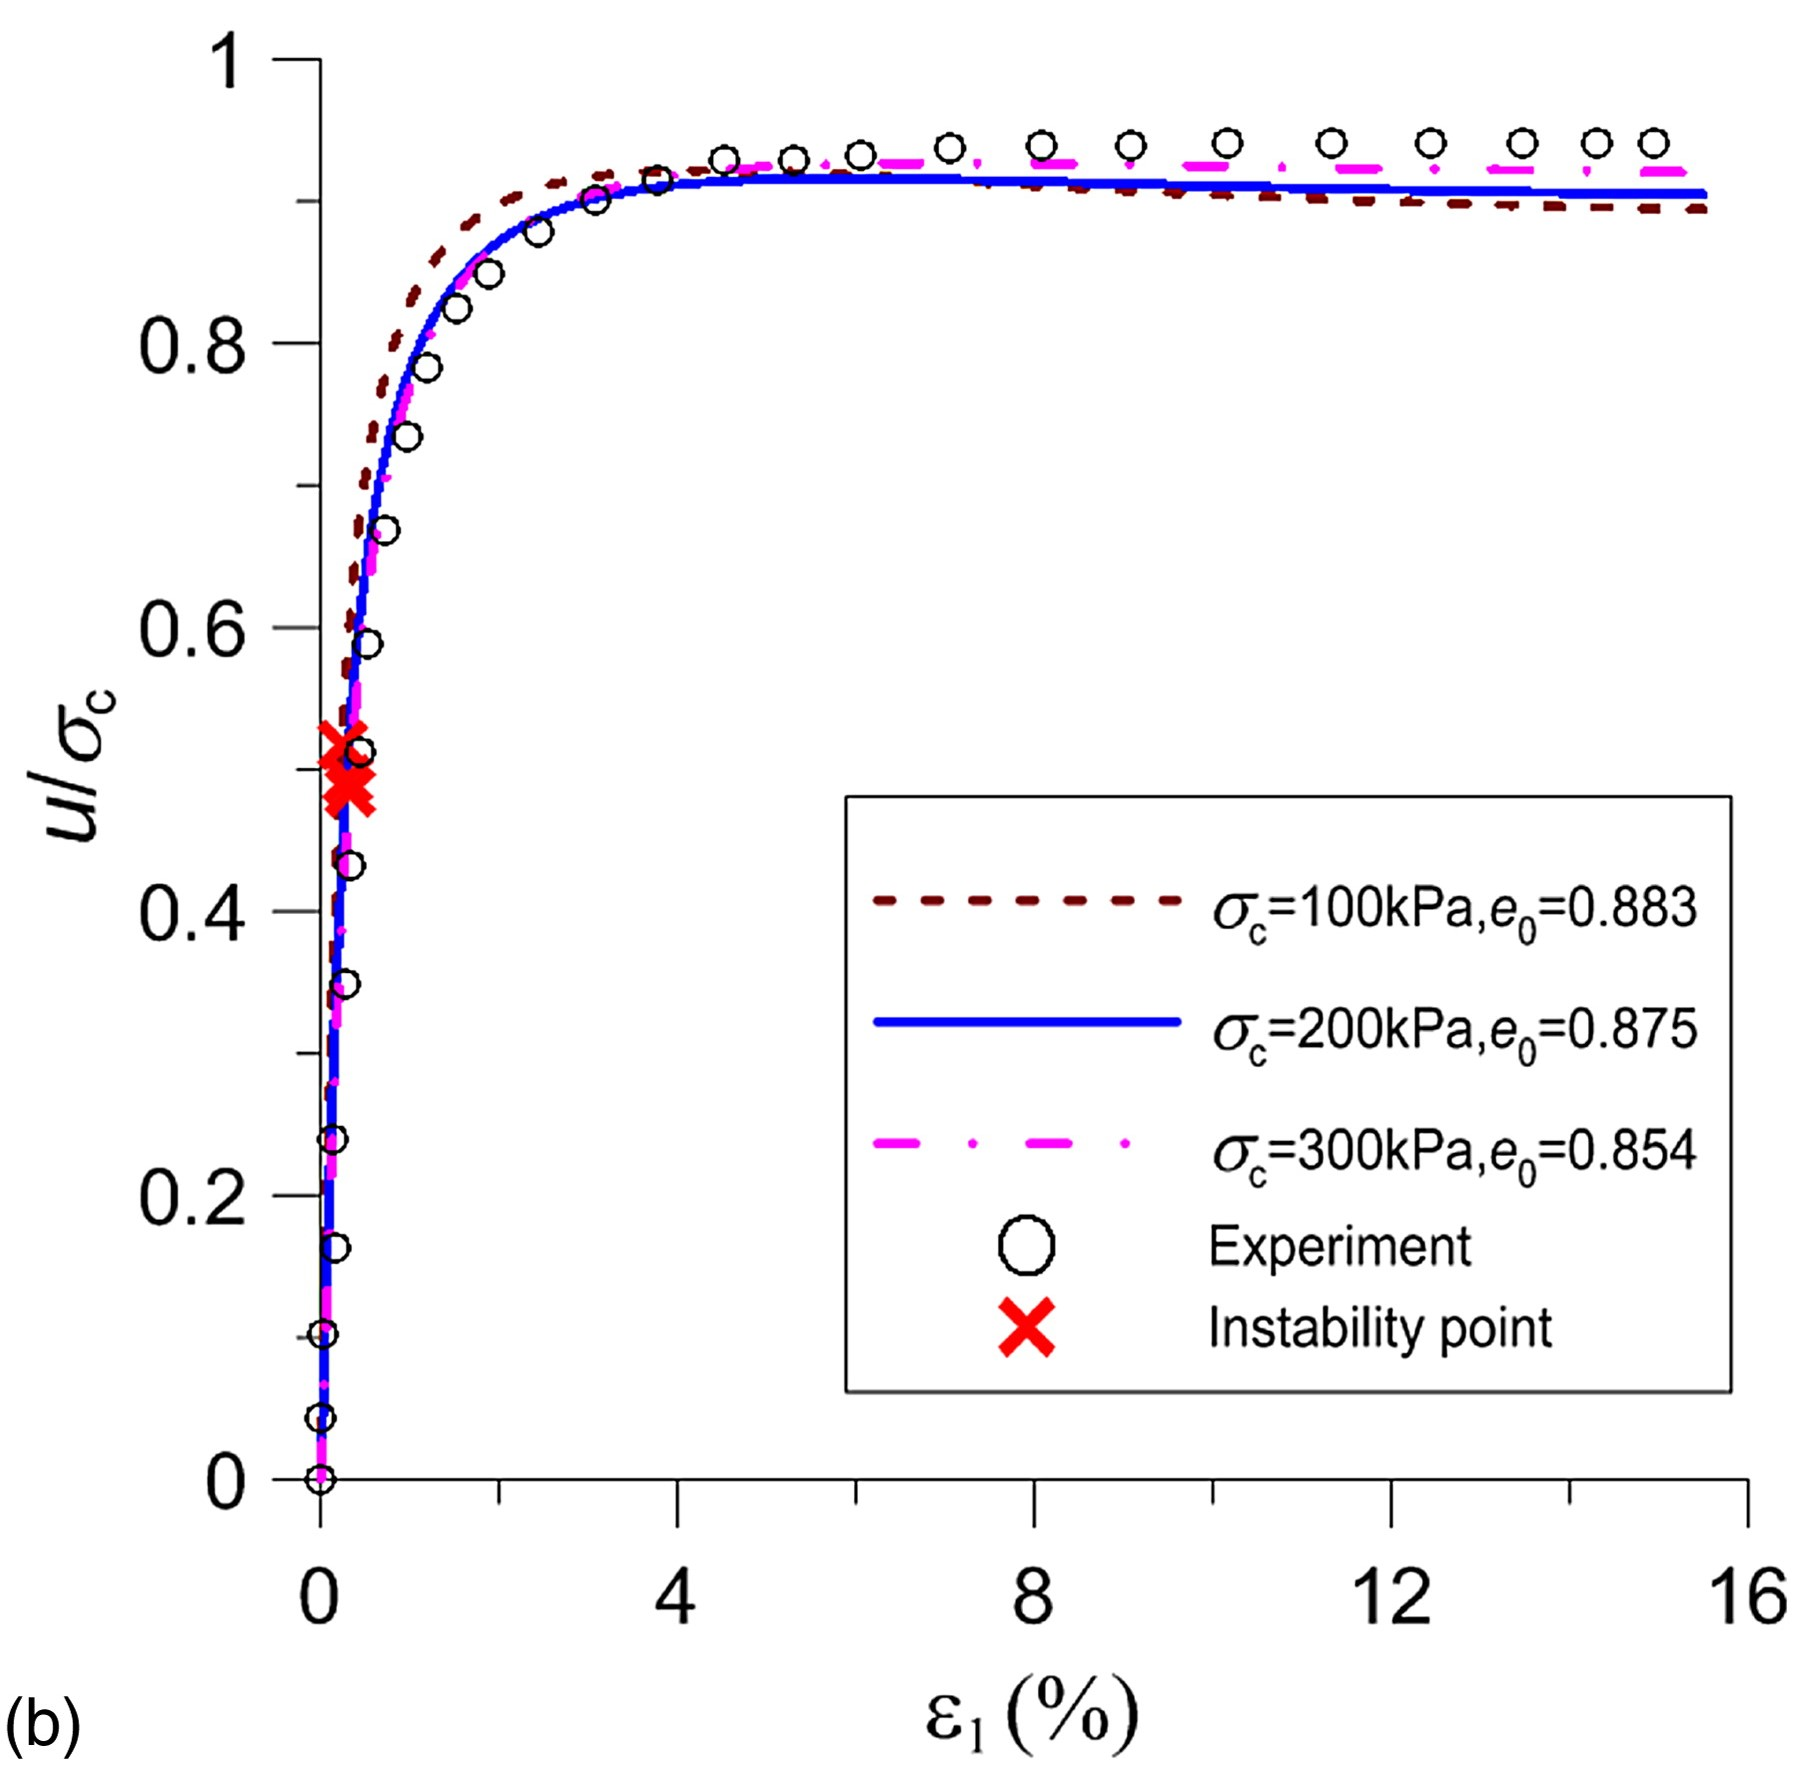
\includegraphics[width=.75\textwidth]{figures/figure5b.jpg}
                \label{figure:5b}
            }
            \bicaption{Model prediction (experimental data from \citealt{Doanh1997})}{模型预测(实验数据来自\citealt{Doanh1997})}
            \label{figure:5}
        \end{figure}
        \begin{figure}[H]
            \centering
            \addtocounter{figure}{1}
            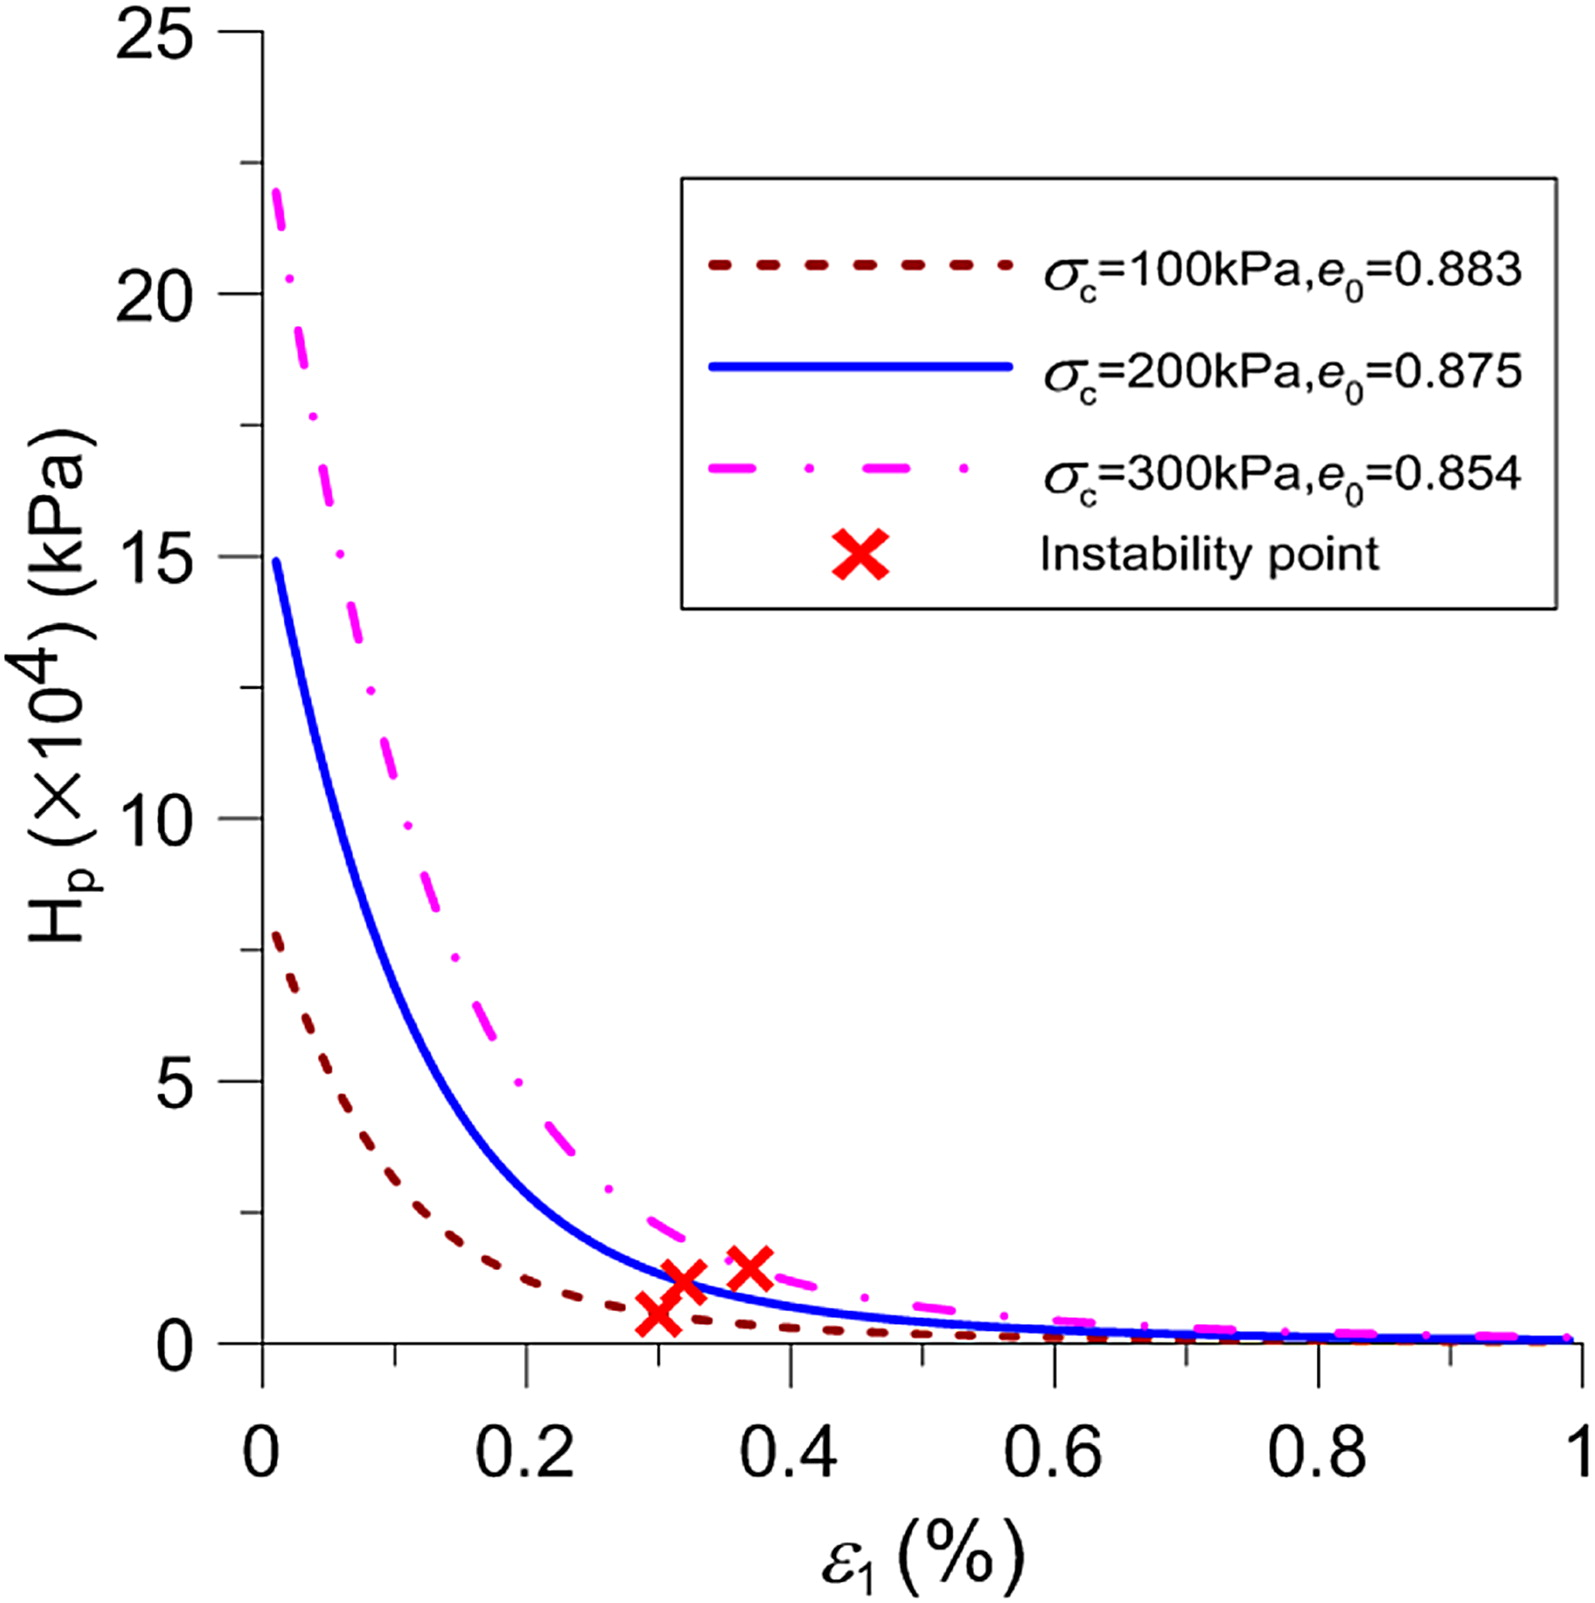
\includegraphics[width=.75\textwidth]{figures/figure7.jpg}
            \bicaption{Evolution of hardening modulus}{硬化模量的演变}
            \label{figure:7}
        \end{figure}
    \end{minipage}
\end{figure}